\documentclass[11pt,a4paper]{scrartcl}

\usepackage[ngerman,english]{babel}
\usepackage{graphicx}
\graphicspath{{pics/}}

\title{Hair Simulation with OpenCL}
\author{Etienne Gramlich \& Heiko Ettwein}


\begin{document}
\maketitle
\tableofcontents
\newpage
\pagenumbering{arabic}

\section{Introduction}
This is a project for the course GPU programming at HTWG Konstanz.

\subsection{Project Description}
This is a hair simulation that runs on the GPU.
The hairs are made of nodes and links between them, then forces (i.e. wind, gravity) are applied to the nodes and are moved accordingly. If the links are stretched they apply a backward force to the nodes.
The forced are applied at each time step in an OpenCL kernel.


\section{Hair Physics}
simple force model, no bounding boxes, small random differences of hair masses

\subsection{Force Model}
acceleration vectors, velocity, mass, linear combination of vectors

\subsubsection{Gravity}
gravitational force

\subsubsection{Elasticity}
link force \\ spring force

\begin{figure}[htbp]
\centering
\fbox{
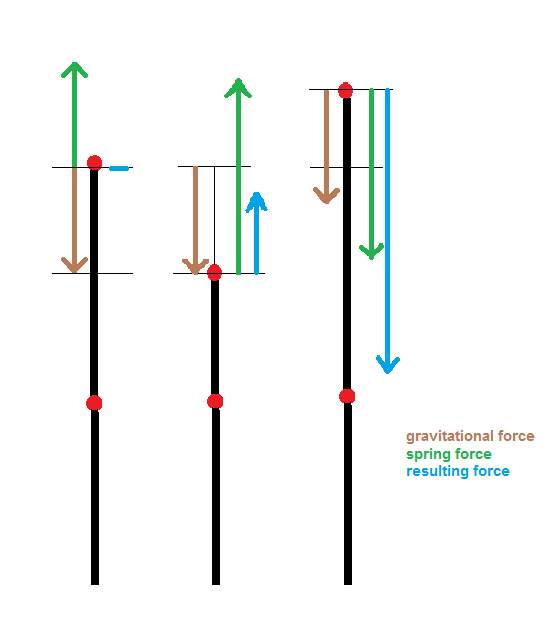
\includegraphics[width=0.8\linewidth]{SpringForce.png}
}
\caption{Spring force}
\end{figure}

\begin{figure}[htbp]
\centering
\fbox{
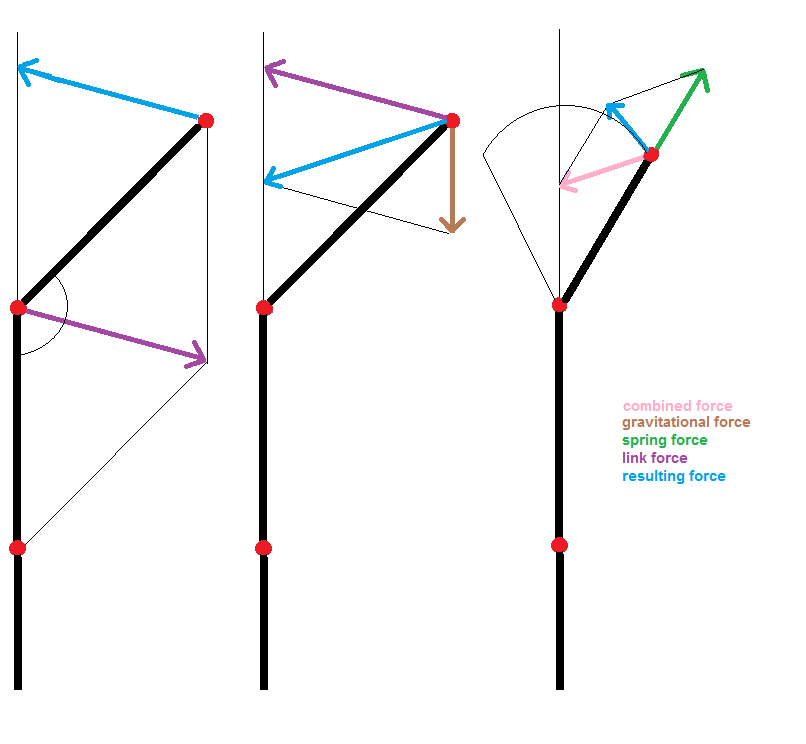
\includegraphics[width=0.8\linewidth]{CombinedForce.png}
}
\caption{Combination of all forces}
\end{figure}


\subsubsection{Wind}
wind force \\ control direction and intensity (maximum force and interval)


\section{Implementation}
The sumulation is implemented in C++ and OpenCL. There are classes for the needed data types: \textit{Vector}, \textit{Node}, \textit{Link} and \textit{HairPiece}. These classes need to have a representation in OpenCL data types. This is trivial for the vector which is a single float3. The other classes have methods to convert instances to OpenCL compatible data types.

The classes \textit{clHelper} and \textit{BodySolver} are the connection to OpenCL, they include simple helper functions and the simulation scheduling for the GPU. \textit{BodySolverCPU} is still present in the repository but not used; it is the CPU implementation of the simulation being used as the template for the implementation in OpenCL. The class \textit{GLwindow} contains the initialization of the window in OpenGL.

\subsection{Classes}
\begin{itemize}
	\item Vector
	\item Node
	\item Link
	\item HairPiece
	\item clHelper
	\item BodySolverCPU
	\item BodySolver
	\item GLwindow
\end{itemize}

\subsubsection{Vector}
This is a class representating a vector in 3D space. It implements some operators like addition (with vector or scalar), length calculation and normalization.
It is used to represent forces, movement and velocities of the nodes.

\subsubsection{Node}
It represents a node of a hair, so it has a position in 3D space, mass, velocity (as Vector class) and may be constant. If it is constant it is prevented from moving, so one side of the hair nodes can be constant so that this side is assumed to be on the surface of another object.

\subsubsection{Link}
This is a link between two nodes and so has 4 elements: one node at each side, the length and a spring constant.

The Spring force is calculated with the distance from the two nodes, the difference o this length to the original link length and the spring constant.

\subsubsection{HairPiece}
HairPiece is a container class for all hairs that belong to one object. It contains a vector with all nodes and one vector with all links.

\subsubsection{clHelper}
This class contains two helper functions to decode OpenCL error codes and print status messages.

\subsubsection{BodySolver}
This class implements the handling of the OpenCL kernel implementing the actual simulation. \textit{BodySolver} contains the nodes and links of the hairs in a \textit{HairPiece} object. The Buffers for copying the nodes and links are created in the constructor, the kernel is compiled there too.

For each time step BodySolver calls the kernel; before that, the nodes and links are converted from CPU data types to OpenCL data thyes and copied to the device. Then the kernel is called, calculated the new positions forces and position of the nodes. Then the nodes are copied back and being converted back to CPU data types. Then the hairs are going to be re-drawn.

\subsubsection{GLwindow}



\subsection{Architecture}

\subsection{OpenCL}

\subsection{OpenGL}


\section{Building}
The program can be built by importing the HairSimulation.sln in Visual Studio 2017 and then builing all sub-projects.

To run the program several files must be copied in the folder where the executable is located: The two shaders in \verb|HairSim\OpenCLProject1\Sample\shader| (fragment.glsl and vertex.glsl) must be places in the same diretory as the executable HairSim.exe. The OpenCL kernel SolvePositionsFromLinksKernel.cl must also be present, but should be copied from Visual Stuidio while building.


\section{Conclusion}


\end{document}